\documentclass[a4paper,titleauthor]{mwart} 

\usepackage{polski}
\usepackage[utf8]{inputenc}
\usepackage{graphicx} %pakiet do wstawiania grafiki
\usepackage[hyphens]{url} %pakiet do wstawiania linkow
%\usepackage[hidelinks,breaklinks]{hyperref}
\usepackage{authblk}%pakiet do tworzenia afiliacji
\usepackage{tabularx}%pakiet do tabel
\usepackage[a4paper, left=2cm, right=2cm, top=3cm, bottom=3cm]{geometry}
\usepackage{listings}
\usepackage{placeins}%pakiet do kontroli umieszczania obiektow
\usepackage{hyperref}%pakiet do m.in. kolorowania linkow

\usepackage[tablegrid,owncaptions]{vhistory}
\renewcommand{\vhhistoryname}{Historia zmian}
\renewcommand{\vhversionname}{Wersja}
\renewcommand{\vhdatename}   {Data}
\renewcommand{\vhauthorname} {Autor}
\renewcommand{\vhchangename} {Opis zmian}

\renewcommand\figurename{Rys.}%skrocony podpis
\renewcommand\lstlistingname{Wydruk}


%------------------------------------------------------------------------
% Dane do strony tytułowej

\title{{\Huge  Projekt SYCYF}\\ - \\{\Large Zespół nr 6}\\ }

\author{Sofiia Levchenko \and Joanna Stalenczyk \and Julia Boryslawska \and Jakub Tarczynski \and Jan Zobniow}

\date{\today}

%------------------------------------------------------------------------
% Początek dokumentu
\begin{document}
	
%Automatycznie generowany tytuł dokumentu
\maketitle
%------------------------------------------------------------------------
% Automatycznie generowany spis treści
\tableofcontents

%------------------------------------------------------------------------
\section{Wstęp}
\label{sec:wstep}%etykieta

Raport bedzie dokumentowany \textbf{przyrostowo} zgodnie z realizacja projektu. Poszczególne etapy realizacji projektu obejmują: 

\renewcommand{\labelenumi}{\Roman{enumi}}
\begin{enumerate}\setlength{\itemsep}{0.2\baselineskip} 
	\item Etap wstępny – stworzenie zespołu i organizacja warsztatu pracy, 
	\item Etap zdobywania informacji – analiza literatury, istniejących metod, zebranie wiedzy teoretycznej związanej z tematem projektu, 
	\item Etap opracowania koncepcji – szukanie rozwiązań, najlepiej sprawdzi się proces burzy mózgów (mapy myśli), opracowanie koncepcji rozwiązania  na podstawie zdobytej wiedzy, opracowanie prostego modelu referencyjnego (Python, MATLAB/GNU Octave, itp) i danych do testowania  
	\item Etap implementacji – na tym etapie rozwijamy i rozbudowujemy koncepcje projektowe docelowego systemu, modelujemy elementy systemu w HDL, weryfikujemy funkcjonalnie, integrujemy i oceniamy prototypy, 
	\item Etap uruchomienia – wdrożenie projektu, uruchomienie na docelowej platformie, przetestowanie według wcześniej opracowanych scenariuszy testowych. 
\end{enumerate}

Prace wykonane w ramach każdego etapu beda opisane w oddzielnych rozdziałach raportu.

\section{Organizacja prac}
\label{sec:organizacja}

Rozdział ten bedzie opisywal zadania zrealizowane w ramach Etapu\texttt{I}. W tym rozdiale beda omowione:

\begin{itemize}
	\item analiza podejscia Design Thinking oraz trzech go wersji (piec krokow Design Thinkig'u, trzy zachodzace na siebie fazy procesu Design Thinking'u oraz cztere-fazowy "Double Dimond" proces)
	\item wybor jedynego sposobu zarządzania projektem
	\item analiza roznego rodzaju narzedzi (TeXstudio, Overleaf, Microsoft Word, Microsoft Teams, Skype, GitHub oraz GitLab)
	\item organizacja warsztatu pracy, dobór narzędzi (Overleaf, Microsoft Teams, GutHub, itp.)
	\item ostateczny dobor narzedzi
	\item organizacja warsztatu pracy
\end{itemize}

\subsection{Design Thinking}
\label{sec:design_thinking}
Co to jest "Design Thinking?" \newline
\newline
Design thinking – to jest proces odnoszący się do procesów poznawczych, strategicznych i praktycznych, dzięki którym koncepcje projektowe (propozycje nowych produktów, usług itp.) są opracowywane przez projektantów i / lub zespoły projektowe~\cite{DesignThinking1}. \newline \newline Spora liczba osob próbowali sformalizować podstawowe zasady zastosowania myślenia projektowego w organizacjach za pomocą modeli procesów i metodologii. Pomimo niekończących się modyfikacji i mutacji istnieją trzy trwałe, ogolne przyjete modele~\cite{DesignThinking2}:

 \begin{itemize}
 	\item Piec krokow Design Thinkig'u
 	\item Trzy zachodzace na siebie fazy procesu Design Thinking'u
 	\item Cztere-fazowy "Double Dimond" proces
 \end{itemize}

Diagramy i słownictwo mogą się różnić, ale we wszystkich modelach myślenia projektowego występują wyraźne tematy:

 \begin{itemize}
	\item \textbf{Zorientowane na człowieka}\newline \newline Fazy odkrywania i inspiracji koncentrują się na badaniach proponowanego użytkownika - "Kim oni są?", "Czego chcą / potrzebują?", "Jak się zachowują?" Chodzi o budowanie empatii przez zespół projektowy z użytkownikiem końcowym i zrozumienie, dla kogo projektują.\newline
	\item \textbf{Iteracyjny} \newline \newline Fazy opracowywania, dostarczania i wdrażania skupiają się na usuwaniu najsłabszych pomysłów i ulepszaniu najsilniejszych poprzez prototypowanie, testowanie i optymalizację.\newline
	\item \textbf{Interdyscyplinarne} \newline \newline Wszystkie modele pokazują podróż, która rozbiega się i zbiega, przynajmniej w początkowe rozwiązanie. Każda faza nie jest własnością jednego zespołu z ustalonymi zadaniami; zamiast tego wspólny zespół projektowy wyrusza razem w podróż. Należy zauważyć, że zespoły interdyscyplinarne różnią się od zespołów multidyscyplinarnych tym, że każdy z nich ma wspólną odpowiedzialność za projekt i jego sukces, zamiast opowiadać się za własną specjalizacją.
 \end{itemize}

Ponizej beda sa przedstawione skrocone opisy, etapy kazdego z danych procesow badz ich wady oraz zalety w wykorzystaniu dla zarzadzania projektem.
 
 \subsubsection{Piec krokow Design Thinkig'u}


 \subsubsection{Trzy zachodzace na siebie fazy procesu Design Thinking'u}
 
Drugim po koleje jest model, ktory sie nazywa "Trzy zachodzace na siebie fazy procesu Design Thinking'u" ~\cite{Proces2}. Jest to proces, ktory zorientowany na człowieka. \newline \newline 
Co to znaczy? \newline \newline
Jest to proces, który rozpoczyna się od osób, dla których projektujesz, a kończy na nowych rozwiązaniach, które są dostosowane i wygenerowane specjalnie do spelnienia ich potrzeb. Projektowanie zorientowane na człowieka polega na budowaniu głębokiej empatii z ludźmi, dla których projektujesz; generowanie ton pomysłów; budowanie wiązki prototypów; dzielenie się tym, co stworzyłeś, z ludźmi, dla których projektujesz; i ostatecznie wypuszczenie na rynek nowego innowacyjnego rozwiązania. \newline \newline
Konstrukcja skoncentrowana na człowieku, w danym procesie, składa się z trzech faz:\newline
 \begin{itemize}
 \item W fazie inspiracji dowiesz się bezpośrednio od ludzi, dla których projektujesz, zanurzając się w ich życiu i dogłębnie rozumiejąc ich potrzeby. 
 \item W fazie idei zrozumiesz, czego się nauczyłeś, zidentyfikujesz możliwości projektowania i prototypujesz możliwe rozwiązania. 
 \item Na etapie wdrażania wprowadzisz swoje rozwiązanie w życie, a ostatecznie na rynek. Będziesz wiedział, że Twoje rozwiązanie odniesie sukces, ponieważ w centrum procesu są ludzie, którym chcesz służyć.
 
 Zobaczyc ilustracje tego procesu mozna na rysunku podanym ponizej.
 
 \begin{figure}[h]
 	\centering
 	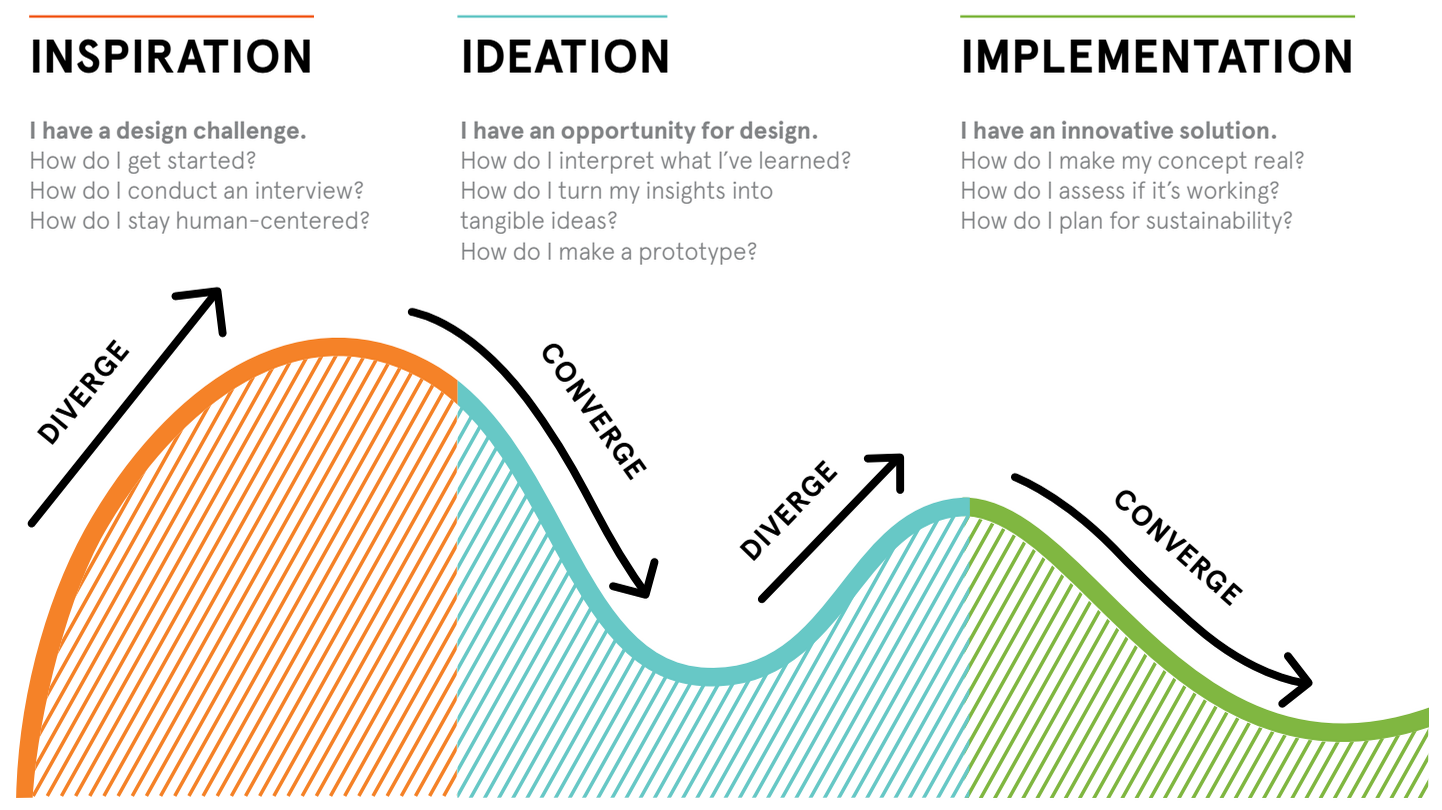
\includegraphics[width=0.8\textwidth]{2}
 	\caption{Trzy zachodzace na siebie fazy procesu Design Thinking'u}
 \end{figure}
 
\end{itemize}

Zalety danego modelu plegaja na:\newline
\begin{itemize}
\item Ulatwia i przyspiesza przyjęcie rozwiązania: dzięki podejściu oddolnemu projektowanie oparte na Design Thinking zaczyna się od potrzeby użytkownika końcowego, aby zbudować rozwiązanie (technologiczne lub procesowe), które jest dla niego naprawdę cenne.
\item Silne zaangażowanie użytkownika końcowego, który czuje się zaangażowany już od strony projektowej: sposób dla firm na ulepszenie swoich pracowników i „wzięcie ich na pokład” stojącego przed nimi wyzwania;
\item Iteracyjne podejście na etapie projektowania pozwala przetestować propozycje rozwiązań i modyfikować je, aż do osiągnięcia najbardziej odpowiedniego rozwiązania przed przystąpieniem do faktycznego wdrożenia;
\end{itemize}
 Wady danego modelu w swoim czasie plegaja na:\newline
\begin{itemize}
	\item Projekt moze trwajc porownajace długo,a koncowa wersję można zastosować tylko do ograniczonych celów
	\item Zastosowanie metodologii projektowania korporacyjnych rozwiązań cyfrowych może kolidować z ograniczeniami nałożonymi przez integrację z już używanymi rozwiazaniami.
	\item Myślenie projektowe wymaga bezpośredniego zaangażowania użytkowników, którzy muszą mieć możliwość wniesienia własnego wkładu (dostępność czasu i zasobów)
\end{itemize}

 \subsubsection{Cztere-fazowy "Double Dimond" proces}

\subsection{Zarządzanie projektem}
\label{sec:zarządzanie_projektem}

\subsubsection{Metody}
\label{sec:narzędzia}

\subsubsection{Narzędzia}
\label{sec:narzędzia}

------------------------------------------------------------
\section{Informacje podstawowe}
\label{sec:informacje_podstawowe}

\section{Koncepcja}
\label{sec:koncepcja}

\section{Implementacja}
\label{sec:implementacja}


\section{Uruchomienie}
\label{sec:uruchomienie}

	
\section{Podsumowanie}
\label{sec:podsumowanie}



\bibliographystyle{plabbrv} % plplain plabbrv plalpha
\begin{thebibliography}{SYCYfProjekt}
\bibitem{DesignThinking1}
 Visser, W. 2006, The cognitive artifacts of designing, Lawrence Erlbaum Associates.
\bibitem{DesignThinking2}
"Design Thinking: A Beginner’s Guide to the History, Terminologies and Methodologies" by Rhoda Sell \url{https://blog.prototypr.io/design-thinking-a-beginners-guide-to-the-history-terminologies-and-methodologies-e527f7afdcd1}
\bibitem{Proces1}
"The five steps of design thinking" by D.School, Stanford University’s Institute of Design \url{https://dschool-old.stanford.edu/sandbox/groups/designresources/wiki/36873/attachments/74b3d/ModeGuideBOOTCAMP2010L.pdf}
\bibitem{Proces2}
"The three overlapping phases of design thinking" by IDEO. \url{https://www.designkit.org/human-centered-design}
\bibitem{Proces3}
"The four-phased ‘Double Diamond’ process" by the Design Council \url{https://www.designcouncil.org.uk/news-opinion/what-framework-innovation-design-councils-evolved-double-diamond}
\end{thebibliography}

\end{document}